%%
% -----------------------------------------------------------------------------
% Trivadis AG, Infrastructure Managed Services
% Saegereistrasse 29, 8152 Glattbrugg, Switzerland
% -----------------------------------------------------------------------------
% Name.......: trivadis.tex
% Author.....: Stefan Oehrli (oes) stefan.oehrli@trivadis.com
% Editor.....: Stefan Oehrli
% Date.......: 2018.11.01
% Revision...: --
% Purpose....: LaTeX template for pandoc
% Notes......: For usage information and examples visit the GitHub page of this 
%              template: https://github.com/oehrlis/pandoc_template
% Reference..: https://github.com/oehrlis/pandoc_template
% License....: GPL-3.0+
% -----------------------------------------------------------------------------
% Modified :
% see git revision history with git log for more information on changes
% -----------------------------------------------------------------------------
%%

\PassOptionsToPackage{unicode=true}{hyperref} % options for packages loaded elsewhere
\PassOptionsToPackage{hyphens}{url}
\PassOptionsToPackage{dvipsnames,svgnames*,table}{xcolor}

\documentclass[a4paper,,tablecaptionabove]{scrartcl}



  \usepackage{lmodern}


\usepackage{amssymb,amsmath}
\usepackage{ifxetex,ifluatex}
\usepackage{fixltx2e} % provides \textsubscript
\ifnum 0\ifxetex 1\fi\ifluatex 1\fi=0 % if pdftex
  \usepackage[T1]{fontenc}
  \usepackage[utf8]{inputenc}
  \usepackage{textcomp} % provides euro and other symbols
\else % if luatex or xelatex

  \usepackage{unicode-math}

\defaultfontfeatures{Ligatures=TeX,Scale=MatchLowercase}


  \setmainfont[]{Nunito Sans SemiBold}


  \setmonofont[Mapping=tex-ansi]{Courier New}



\fi


% use upquote if available, for straight quotes in verbatim environments
\IfFileExists{upquote.sty}{\usepackage{upquote}}{}

% use microtype if available
\IfFileExists{microtype.sty}{%
  \usepackage[]{microtype}
  \UseMicrotypeSet[protrusion]{basicmath} % disable protrusion for tt fonts
}{}

  \IfFileExists{parskip.sty}{%
    \usepackage{parskip}
  }{% else
    \setlength{\parindent}{0pt}
    \setlength{\parskip}{6pt plus 2pt minus 1pt}
  }



\usepackage{titlesec}
\newcommand{\sectionbreak}{\clearpage}
\usepackage{hyperref}
\hypersetup{
      pdftitle={EUS, Kerberos, SSL and OUD a guideline},
        pdfauthor={Stefan Oehrli},
            pdfborder={0 0 0},
    breaklinks=true}

\urlstyle{same}  % don't use monospace font for urls

  \usepackage[margin=2.5cm,includehead=true,includefoot=true,centering]{geometry}

% load graphicx any way
  \usepackage[export]{adjustbox}
  \usepackage{graphicx}




  \usepackage{color}
  \usepackage{fancyvrb}
  \newcommand{\VerbBar}{|}
  \newcommand{\VERB}{\Verb[commandchars=\\\{\}]}
  \DefineVerbatimEnvironment{Highlighting}{Verbatim}{commandchars=\\\{\}}
  % Add ',fontsize=\small' for more characters per line
  \newenvironment{Shaded}{}{}
  \newcommand{\AlertTok}[1]{\textcolor[rgb]{1.00,0.00,0.00}{\textbf{#1}}}
  \newcommand{\AnnotationTok}[1]{\textcolor[rgb]{0.38,0.63,0.69}{\textbf{\textit{#1}}}}
  \newcommand{\AttributeTok}[1]{\textcolor[rgb]{0.49,0.56,0.16}{#1}}
  \newcommand{\BaseNTok}[1]{\textcolor[rgb]{0.25,0.63,0.44}{#1}}
  \newcommand{\BuiltInTok}[1]{#1}
  \newcommand{\CharTok}[1]{\textcolor[rgb]{0.25,0.44,0.63}{#1}}
  \newcommand{\CommentTok}[1]{\textcolor[rgb]{0.38,0.63,0.69}{\textit{#1}}}
  \newcommand{\CommentVarTok}[1]{\textcolor[rgb]{0.38,0.63,0.69}{\textbf{\textit{#1}}}}
  \newcommand{\ConstantTok}[1]{\textcolor[rgb]{0.53,0.00,0.00}{#1}}
  \newcommand{\ControlFlowTok}[1]{\textcolor[rgb]{0.00,0.44,0.13}{\textbf{#1}}}
  \newcommand{\DataTypeTok}[1]{\textcolor[rgb]{0.56,0.13,0.00}{#1}}
  \newcommand{\DecValTok}[1]{\textcolor[rgb]{0.25,0.63,0.44}{#1}}
  \newcommand{\DocumentationTok}[1]{\textcolor[rgb]{0.73,0.13,0.13}{\textit{#1}}}
  \newcommand{\ErrorTok}[1]{\textcolor[rgb]{1.00,0.00,0.00}{\textbf{#1}}}
  \newcommand{\ExtensionTok}[1]{#1}
  \newcommand{\FloatTok}[1]{\textcolor[rgb]{0.25,0.63,0.44}{#1}}
  \newcommand{\FunctionTok}[1]{\textcolor[rgb]{0.02,0.16,0.49}{#1}}
  \newcommand{\ImportTok}[1]{#1}
  \newcommand{\InformationTok}[1]{\textcolor[rgb]{0.38,0.63,0.69}{\textbf{\textit{#1}}}}
  \newcommand{\KeywordTok}[1]{\textcolor[rgb]{0.00,0.44,0.13}{\textbf{#1}}}
  \newcommand{\NormalTok}[1]{#1}
  \newcommand{\OperatorTok}[1]{\textcolor[rgb]{0.40,0.40,0.40}{#1}}
  \newcommand{\OtherTok}[1]{\textcolor[rgb]{0.00,0.44,0.13}{#1}}
  \newcommand{\PreprocessorTok}[1]{\textcolor[rgb]{0.74,0.48,0.00}{#1}}
  \newcommand{\RegionMarkerTok}[1]{#1}
  \newcommand{\SpecialCharTok}[1]{\textcolor[rgb]{0.25,0.44,0.63}{#1}}
  \newcommand{\SpecialStringTok}[1]{\textcolor[rgb]{0.73,0.40,0.53}{#1}}
  \newcommand{\StringTok}[1]{\textcolor[rgb]{0.25,0.44,0.63}{#1}}
  \newcommand{\VariableTok}[1]{\textcolor[rgb]{0.10,0.09,0.49}{#1}}
  \newcommand{\VerbatimStringTok}[1]{\textcolor[rgb]{0.25,0.44,0.63}{#1}}
  \newcommand{\WarningTok}[1]{\textcolor[rgb]{0.38,0.63,0.69}{\textbf{\textit{#1}}}}

\usepackage{longtable,booktabs,tabularx}
      % Fix footnotes in tables (requires footnote package)
    \IfFileExists{footnote.sty}{\usepackage{footnote}\makesavenoteenv{longtable}}{}
  
  \usepackage{graphicx,grffile}
  \makeatletter
  \def\maxwidth{\ifdim\Gin@nat@width>\linewidth\linewidth\else\Gin@nat@width\fi}
  \def\maxheight{\ifdim\Gin@nat@height>\textheight\textheight\else\Gin@nat@height\fi}
  \makeatother
  % Scale images if necessary, so that they will not overflow the page
  % margins by default, and it is still possible to overwrite the defaults
  % using explicit options in \includegraphics[width, height, ...]{}
  \setkeys{Gin}{width=\maxwidth,height=\maxheight,keepaspectratio}



\setlength{\emergencystretch}{3em}  % prevent overfull lines
\providecommand{\tightlist}{\setlength{\itemsep}{0pt}\setlength{\parskip}{0pt}}

  \setcounter{secnumdepth}{5}

      % Redefines (sub)paragraphs to behave more like sections
    \ifx\paragraph\undefined\else
    \let\oldparagraph\paragraph
    \renewcommand{\paragraph}[1]{\oldparagraph{#1}\mbox{}}
    \fi
    \ifx\subparagraph\undefined\else
    \let\oldsubparagraph\subparagraph
    \renewcommand{\subparagraph}[1]{\oldsubparagraph{#1}\mbox{}}
    \fi
  

% Make use of float-package and set default placement for figures to H
\usepackage{float}
\floatplacement{figure}{H}






  \title{EUS, Kerberos, SSL and OUD a guideline\thanks{Hans, Fritz, meiner Frau und der Familie}}

  \providecommand{\subtitle}[1]{}
  \subtitle{Demo Scripts, Examples and Exercises}

  \author{Stefan Oehrli}

\date{2018 November 01}


%% - Begin added ---------------------------------------------------------
% No language specified? take American English.
  \ifnum 0\ifxetex 1\fi\ifluatex 1\fi=0 % if pdftex
    \usepackage[shorthands=off,main=english]{babel}
      \else
            % load polyglossia as late as possible as it *could* call bidi if RTL lang (e.g. Hebrew or Arabic)
    \usepackage{polyglossia}
    \setmainlanguage[]{english}
      \fi

%
% colors
\usepackage[]{xcolor}

%
% Trivadis colors
\definecolor{tvdgray}{gray}{0.9}
\definecolor{tvdgray2}{gray}{0.8}
\definecolor{tvdred}{RGB}{204,0,0}
\definecolor{tvdyellow}{RGB}{255,128,0}
\definecolor{tvdgreen}{RGB}{51,192,0}

% listing colors
\definecolor{listing-background}{HTML}{F7F7F7}
\definecolor{listing-rule}{HTML}{B3B2B3}
\definecolor{listing-numbers}{HTML}{B3B2B3}
\definecolor{listing-text-color}{HTML}{000000}
\definecolor{listing-keyword}{HTML}{435489}
\definecolor{listing-identifier}{HTML}{435489}
\definecolor{listing-string}{HTML}{00999A}
\definecolor{listing-comment}{HTML}{8E8E8E}
\definecolor{listing-javadoc-comment}{HTML}{006CA9}

% for the background color of the title page  
  % make use of textpos package
  \usepackage[absolute]{textpos}
  \usepackage{pagecolor}
  \usepackage{afterpage}

% TOC depth and 
% section numbering depth
\setcounter{tocdepth}{3}
  \setcounter{secnumdepth}{3}

% line spacing
  \usepackage{setspace}
  \setstretch{1.2}

% break urls
\PassOptionsToPackage{hyphens}{url}

% When using babel or polyglossia with biblatex, loading csquotes is recommended 
% to ensure that quoted texts are typeset according to the rules of your main language.
%
\usepackage{csquotes}

% captions
\definecolor{caption-color}{HTML}{777777}
\usepackage[font={stretch=1.2}, textfont={color=caption-color}, position=top, skip=4mm, labelfont=bf, singlelinecheck=false, justification=raggedright]{caption}
\setcapindent{0em}
\captionsetup[longtable]{position=above}

% blockquote
\definecolor{blockquote-border}{RGB}{221,221,221}
\definecolor{blockquote-text}{RGB}{119,119,119}
\usepackage{mdframed}
\newmdenv[rightline=false,bottomline=false,topline=false,linewidth=3pt,linecolor=blockquote-border,skipabove=\parskip]{customblockquote}
\renewenvironment{quote}{\begin{customblockquote}\list{}{\rightmargin=0em\leftmargin=0em}%
\item\relax\color{blockquote-text}\ignorespaces}{\unskip\unskip\endlist\end{customblockquote}}

% Source Sans Pro as the de­fault font fam­ily
% Source Code Pro for monospace text
%
% 'default' option sets the default 
% font family to Source Sans Pro, not \sfdefault.
%

% heading color
\definecolor{heading-color}{RGB}{40,40,40}
\addtokomafont{section}{\color{heading-color}}
% When using the classes report, scrreprt, book, 
% scrbook or memoir, uncomment the following line.
%\addtokomafont{chapter}{\color{heading-color}}

% variables for title and author
\usepackage{titling}
\title{EUS, Kerberos, SSL and OUD a guideline}
\author{Stefan Oehrli}

% tables
\definecolor{table-row-color}{gray}{0.8}
\definecolor{table-rule-color}{gray}{0.8}

\arrayrulecolor{black}
%%\arrayrulecolor{table-rule-color}     % color of \toprule, \midrule, \bottomrule
%\arrayrulecolor{tvdgray2}     % color of \toprule, \midrule, \bottomrule
\setlength\heavyrulewidth{0.3ex}      % thickness of \toprule, \bottomrule
\renewcommand{\arraystretch}{1.3}     % spacing (padding)

  % Reset rownum counter so that each table
  % starts with the same row colors.
  % https://tex.stackexchange.com/questions/170637/restarting-rowcolors
  \let\oldlongtable\longtable
  \let\endoldlongtable\endlongtable
  \renewenvironment{longtable}{
  %\rowcolors{3}{}{table-row-color!100}  % row color
  \oldlongtable} {
    \endoldlongtable
\global\rownum=0\relax}

  % Unfortunately the colored cells extend beyond the edge of the 
  % table because pandoc uses @-expressions (@{}) like so: 
  %
  % \begin{longtable}[]{@{}ll@{}}
  % \end{longtable}
  %
  % https://en.wikibooks.org/wiki/LaTeX/Tables#.40-expressions

% remove paragraph indention
\setlength{\parindent}{0pt}
\setlength{\parskip}{6pt plus 2pt minus 1pt}
\setlength{\emergencystretch}{3em}  % prevent overfull lines

% Listings

% header and footer
  \usepackage{fancyhdr}
  \usepackage{lastpage}
  \pagestyle{fancy}
  \fancyhead{}
  \fancyfoot{}

  \newcommand*{\TVDLogo}{
\includegraphics[width=0.2\textwidth]{images/TVDLogo2019.eps}}

  \lhead[ \TVDLogo ]{}
  \chead[]{}
  \rhead[]{ \TVDLogo }

  \lfoot[\thepage\ / \pageref*{LastPage}]{EUS, Kerberos, SSL and OUD a guideline}
  \cfoot[]{}
  \rfoot[EUS, Kerberos, SSL and OUD a guideline]{\thepage\ / \pageref*{LastPage}}

  \renewcommand{\headrulewidth}{0.4pt}
  \renewcommand{\footrulewidth}{0.4pt}

%% - End added -----------------------------------------------------------

%% - Begin Document ------------------------------------------------------
\begin{document}
%% - Begin titlepage -----------------------------------------------------
  %\thispagestyle{fancyplain2}
  \begin{titlepage}
  
  % TVD Boxes
  \begin{flushleft}
  %  \color{tvdred}\rule{2,5cm}{2,5cm} \hspace{2mm} \color{tvdgray}\rule{2,5cm}{2,5cm} \hspace{2mm} \rule{2,5cm}{2,5cm} 
  \end{flushleft}

      \begin{flushright}
      
\includegraphics[width=5.12cm, right]{images/TVDLogo2019.eps}
    \end{flushright}
  
  \begin{flushright}
    \vfill
    \noindent {\huge \textbf{\textsf{EUS, Kerberos, SSL and OUD a guideline}}}\\
        \bigskip
      {\Large \textsf{Demo Scripts, Examples and Exercises}}\\
    
    \bigskip

    \begin{flushright}
      \textbf{ 
        2018 November 01,
        Version 0.9 }\\
    \end{flushright}
    \vfill
  \end{flushright}

  %% TVD Location
  \begin{flushright}
     \textit{Trivadis AG\\} 
     \textit{Sägereistrasse 29\\} 
     \textit{8152} 
     \textit{Glattbrugg} 
    \par
  \end{flushright}

  %% TVD Contact
  \begin{flushright}
    
    
     \textit{info@trivadis.com\\} 
     \textit{+41 58 459 55 55\\} 
  \end{flushright}
  \end{titlepage}
%% - End Titlepage -------------------------------------------------------

    

  
      {
            \setcounter{tocdepth}{3}
      \tableofcontents
              \newpage
          }
  
  \listoftables

  \listoffigures

\hypertarget{demos-eus-kerberos-ssl-and-oud-a-guideline}{%
\section{Demos EUS, Kerberos, SSL and OUD a
guideline}\label{demos-eus-kerberos-ssl-and-oud-a-guideline}}

A couple of demo's for the TechEvent presentation \emph{EUS, Kerberos,
SSL and OUD a guideline}. Be aware, that the code can not be used
copy/past in all environments due to limitations on the line breaks.

Demos are shown on an Oracle 18c Docker based database.

\begin{Shaded}
\begin{Highlighting}[]
\ExtensionTok{docker}\NormalTok{ run --detach --name te2018_eusdb \textbackslash{}}
\NormalTok{  --volume /data/docker/volumes/te2018_eusdb:/u01 \textbackslash{}}
\NormalTok{  -e ORACLE_SID=TE18EUS \textbackslash{}}
\NormalTok{  -p 1521:1521 -p 5500:5500 \textbackslash{}}
\NormalTok{  --hostname te2018_eusdb.postgasse.org \textbackslash{}}
\NormalTok{  --dns 192.168.56.70 \textbackslash{}}
\NormalTok{  --dns-search postgasse.org \textbackslash{}}
\NormalTok{  oracle/database:18.3.0.0}
\end{Highlighting}
\end{Shaded}

Create user and roles

\begin{Shaded}
\begin{Highlighting}[]
\KeywordTok{CREATE} \KeywordTok{ROLE}\NormalTok{ tvd_connect;}
\KeywordTok{GRANT} \KeywordTok{CREATE} \KeywordTok{SESSION} \KeywordTok{TO}\NormalTok{ tvd_connect;}
\KeywordTok{GRANT} \KeywordTok{select} \KeywordTok{ON}\NormalTok{ v_$session }\KeywordTok{TO}\NormalTok{ tvd_connect;}
\KeywordTok{CREATE} \FunctionTok{USER}\NormalTok{ SOE_KERBEROS }\KeywordTok{IDENTIFIED} \KeywordTok{EXTERNALLY} \KeywordTok{AS} \StringTok{'soe@POSTGASSE.ORG'}\NormalTok{;}
\KeywordTok{GRANT}\NormalTok{ tvd_connect }\KeywordTok{TO}\NormalTok{ SOE_KERBEROS;}
\end{Highlighting}
\end{Shaded}

\begin{longtable}[]{@{}lll@{}}
\toprule
ID & Test & Comment\tabularnewline
\midrule
\endhead
1 & wieso & halt Here's a sentence with a footnote. \footnote{This is
  the footnote.}\tabularnewline
2 & wieso & halt text \footnote{temehrst.}\tabularnewline
3 & wieso & halt text\tabularnewline
4 & wieso & halt text\tabularnewline
5 & wieso & halt text\tabularnewline
\bottomrule
\end{longtable}

etwas test dazwischen

\begin{longtable}[]{@{}llllll@{}}
\toprule
Version & Windows & HPUX & AIX & Solaris & Linux 64bit\tabularnewline
\midrule
\endhead
RDBMS 18.1.0.0 & & n/a & & &\tabularnewline
RDBMS 18.2.0.0 & & n/a & \textbf{Ok} & &
\textbf{\emph{Ok}}\tabularnewline
RDBMS 18.3.0.0 & & n/a & & 
\includegraphics{images/nok.png}
&\tabularnewline
RDBMS 18.3.0.0 & & & & 
\includegraphics{images/ok.png} &\tabularnewline
RDBMS 18.1.0.0 & & & 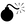
\includegraphics{images/crash.png}\footnote{known
  issue regarding MOS Note XYZ} & &\tabularnewline
\bottomrule
\end{longtable}

Here's a sentence with a footnote. \footnote{wieso}

ein Bild zum Anschauen

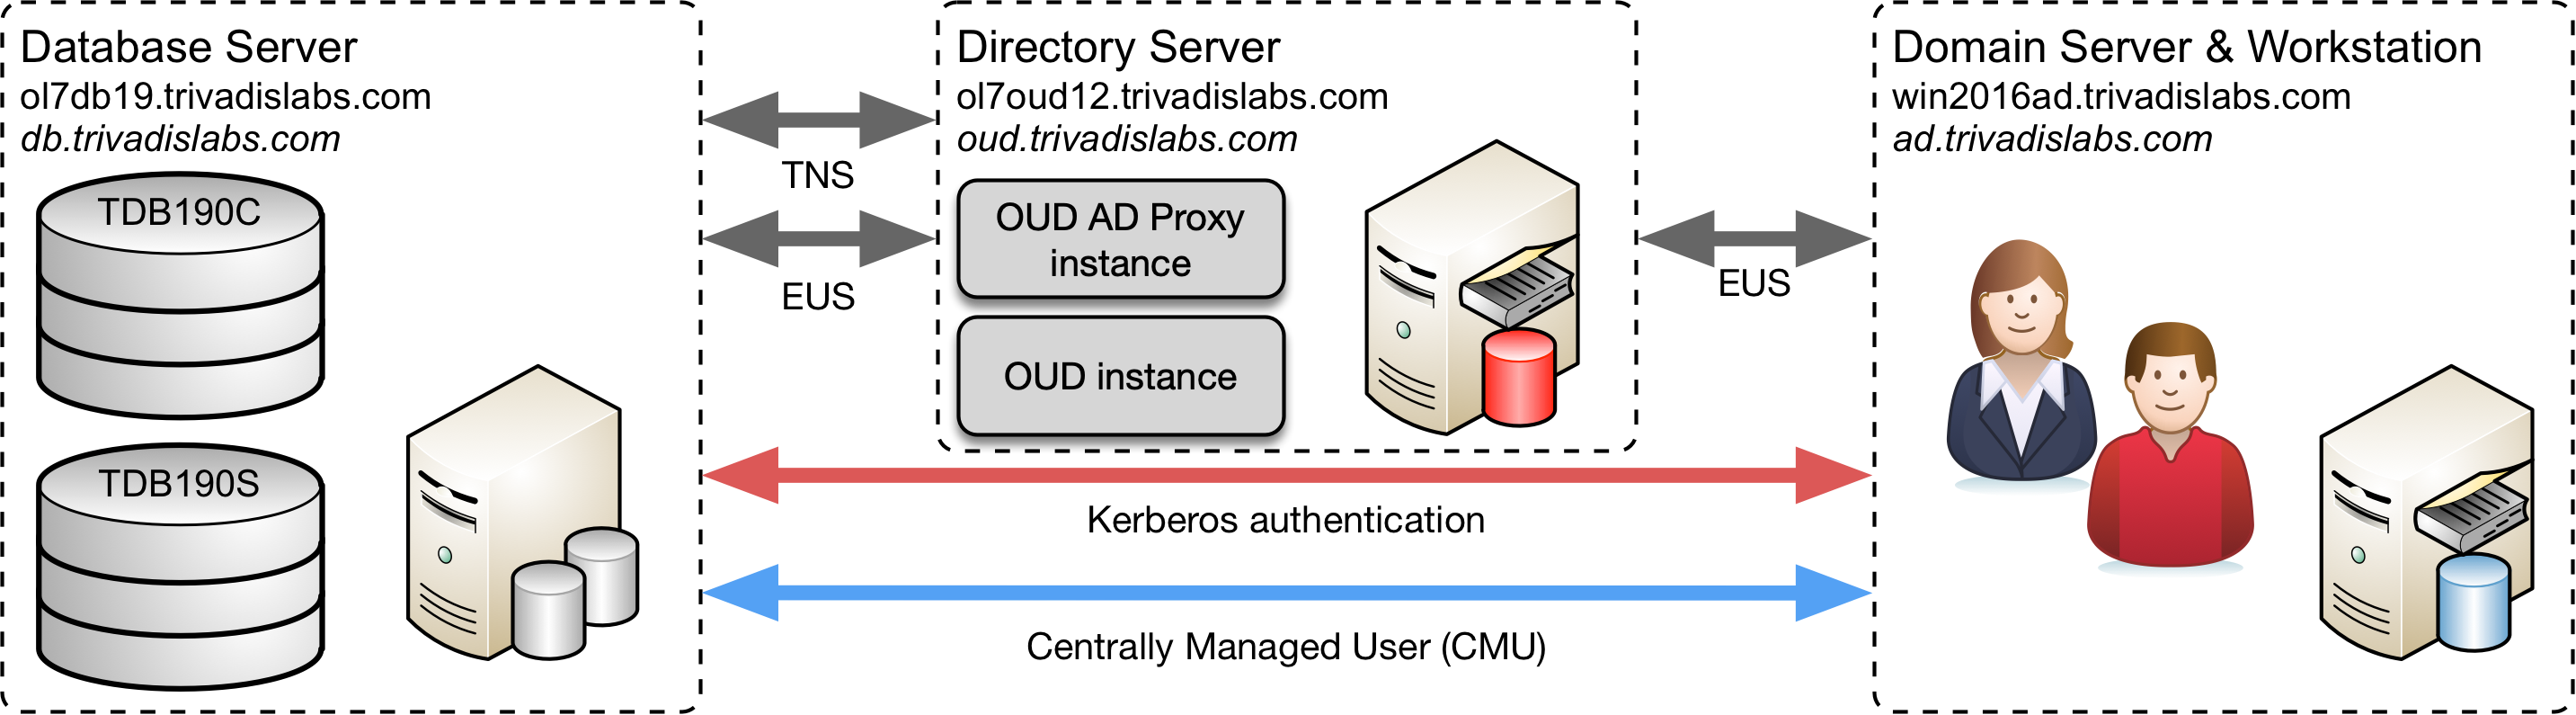
\includegraphics{examples/images/LabEnvironment.png} \emph{Abb. 1:
Architektur Lab Umgebung}

\hypertarget{password-verifier}{%
\subsection{Password Verifier}\label{password-verifier}}

Clean up and remove the old users.

\begin{Shaded}
\begin{Highlighting}[]
\KeywordTok{DROP} \FunctionTok{USER}\NormalTok{ user_10g;}
\KeywordTok{DROP} \FunctionTok{USER}\NormalTok{ user_11g;}
\KeywordTok{DROP} \FunctionTok{USER}\NormalTok{ user_12c;}
\KeywordTok{DROP} \FunctionTok{USER}\NormalTok{ user_all;}
\end{Highlighting}
\end{Shaded}

Create 4 dedicated test user and grant them \emph{CREATE SESSION}.

\begin{Shaded}
\begin{Highlighting}[]
\KeywordTok{GRANT} \KeywordTok{CREATE} \KeywordTok{SESSION} \KeywordTok{TO}\NormalTok{ user_10g }\KeywordTok{IDENTIFIED} \KeywordTok{BY}\NormalTok{ manager;}
\KeywordTok{GRANT} \KeywordTok{CREATE} \KeywordTok{SESSION} \KeywordTok{TO}\NormalTok{ user_11g }\KeywordTok{IDENTIFIED} \KeywordTok{BY}\NormalTok{ manager;}
\KeywordTok{GRANT} \KeywordTok{CREATE} \KeywordTok{SESSION} \KeywordTok{TO}\NormalTok{ user_12c }\KeywordTok{IDENTIFIED} \KeywordTok{BY}\NormalTok{ manager;}
\KeywordTok{GRANT} \KeywordTok{CREATE} \KeywordTok{SESSION} \KeywordTok{TO}\NormalTok{ user_all }\KeywordTok{IDENTIFIED} \KeywordTok{BY}\NormalTok{ manager;}
\end{Highlighting}
\end{Shaded}

Reset all passwords using \emph{IDENTIFIED BY VALUES} to explicitly set
a particular password verifier.

\begin{Shaded}
\begin{Highlighting}[]
\KeywordTok{ALTER} \FunctionTok{USER}\NormalTok{ user_10g }\KeywordTok{IDENTIFIED} \KeywordTok{BY} \KeywordTok{VALUES} \StringTok{'808E79166793CFD1'}\NormalTok{;}
\KeywordTok{ALTER} \FunctionTok{USER}\NormalTok{ user_11g }\KeywordTok{IDENTIFIED} \KeywordTok{BY} \KeywordTok{VALUES} \StringTok{'S:22D8239017006EBDE054108BF367F}
\StringTok{                                        225B5E731D12C91A3BEB31FA28D4A38'}\NormalTok{;}
\KeywordTok{ALTER} \FunctionTok{USER}\NormalTok{ user_12c }\KeywordTok{IDENTIFIED} \KeywordTok{BY} \KeywordTok{VALUES} \StringTok{'T:C6CE7A88CC5D0E048F32A564D2B6A7}
\StringTok{                                        BDC78A2092184F28D13A90FC071F804E5E}
\StringTok{                                        A09D4D2A3749AA79BFD0A90D18DEC5788D}
\StringTok{                                        2B8754AE20EE5C309DBA87550E8AA15EAF}
\StringTok{                                        2746ED431BF4543D2ABE33E22678'}\NormalTok{;}
\end{Highlighting}
\end{Shaded}

an other table

\begin{longtable}[]{@{}llllll@{}}
\toprule
\begin{minipage}[b]{0.03\columnwidth}\raggedright
\#\strut
\end{minipage} & \begin{minipage}[b]{0.74\columnwidth}\raggedright
Description\strut
\end{minipage} & \begin{minipage}[b]{0.01\columnwidth}\raggedright
L1\strut
\end{minipage} & \begin{minipage}[b]{0.01\columnwidth}\raggedright
L2\strut
\end{minipage} & \begin{minipage}[b]{0.01\columnwidth}\raggedright
L3\strut
\end{minipage} & \begin{minipage}[b]{0.02\columnwidth}\raggedright
Since\strut
\end{minipage}\tabularnewline
\midrule
\endhead
\begin{minipage}[t]{0.03\columnwidth}\raggedright
\textbf{1.1}\strut
\end{minipage} & \begin{minipage}[t]{0.74\columnwidth}\raggedright
Verify that technical employees (especially the ones tasked with DevOps
like activities and architects) receive regular training on security
aspects of the technologies they use.\strut
\end{minipage} & \begin{minipage}[t]{0.01\columnwidth}\raggedright
\strut
\end{minipage} & \begin{minipage}[t]{0.01\columnwidth}\raggedright
\strut
\end{minipage} & \begin{minipage}[t]{0.01\columnwidth}\raggedright
\strut
\end{minipage} & \begin{minipage}[t]{0.02\columnwidth}\raggedright
1.0\strut
\end{minipage}\tabularnewline
\begin{minipage}[t]{0.03\columnwidth}\raggedright
\textbf{1.2}\strut
\end{minipage} & \begin{minipage}[t]{0.74\columnwidth}\raggedright
Verify that managers receive regular training on security aspects of the
technologies used in their projects.\strut
\end{minipage} & \begin{minipage}[t]{0.01\columnwidth}\raggedright
\strut
\end{minipage} & \begin{minipage}[t]{0.01\columnwidth}\raggedright
\strut
\end{minipage} & \begin{minipage}[t]{0.01\columnwidth}\raggedright
\strut
\end{minipage} & \begin{minipage}[t]{0.02\columnwidth}\raggedright
1.0\strut
\end{minipage}\tabularnewline
\begin{minipage}[t]{0.03\columnwidth}\raggedright
\textbf{1.3}\strut
\end{minipage} & \begin{minipage}[t]{0.74\columnwidth}\raggedright
Verify that all handled data is classified based on internal data
classification standards.\strut
\end{minipage} & \begin{minipage}[t]{0.01\columnwidth}\raggedright
\strut
\end{minipage} & \begin{minipage}[t]{0.01\columnwidth}\raggedright
\strut
\end{minipage} & \begin{minipage}[t]{0.01\columnwidth}\raggedright
\strut
\end{minipage} & \begin{minipage}[t]{0.02\columnwidth}\raggedright
1.0\strut
\end{minipage}\tabularnewline
\begin{minipage}[t]{0.03\columnwidth}\raggedright
\textbf{1.4}\strut
\end{minipage} & \begin{minipage}[t]{0.74\columnwidth}\raggedright
Verify that each service/application (can consist of multiple
containers) has a security concept which provides information on the
security needs of the service/application and how they are or will be
addressed.\strut
\end{minipage} & \begin{minipage}[t]{0.01\columnwidth}\raggedright
\strut
\end{minipage} & \begin{minipage}[t]{0.01\columnwidth}\raggedright
\strut
\end{minipage} & \begin{minipage}[t]{0.01\columnwidth}\raggedright
\strut
\end{minipage} & \begin{minipage}[t]{0.02\columnwidth}\raggedright
1.0\strut
\end{minipage}\tabularnewline
\begin{minipage}[t]{0.03\columnwidth}\raggedright
\textbf{1.5}\strut
\end{minipage} & \begin{minipage}[t]{0.74\columnwidth}\raggedright
Verify that identified security risks and vulnerabilities are promptly
eliminated (or an exception is granted) and centrally managed according
to a predefined risk and vulnerability management process.\strut
\end{minipage} & \begin{minipage}[t]{0.01\columnwidth}\raggedright
\strut
\end{minipage} & \begin{minipage}[t]{0.01\columnwidth}\raggedright
\strut
\end{minipage} & \begin{minipage}[t]{0.01\columnwidth}\raggedright
\strut
\end{minipage} & \begin{minipage}[t]{0.02\columnwidth}\raggedright
1.0\strut
\end{minipage}\tabularnewline
\begin{minipage}[t]{0.03\columnwidth}\raggedright
\textbf{1.6}\strut
\end{minipage} & \begin{minipage}[t]{0.74\columnwidth}\raggedright
Verify the roles and responsibilities concerning the container
infrastructure are defined. This includes e.g.~who approves connectivity
or decides on allowed base images.\strut
\end{minipage} & \begin{minipage}[t]{0.01\columnwidth}\raggedright
\strut
\end{minipage} & \begin{minipage}[t]{0.01\columnwidth}\raggedright
\strut
\end{minipage} & \begin{minipage}[t]{0.01\columnwidth}\raggedright
\strut
\end{minipage} & \begin{minipage}[t]{0.02\columnwidth}\raggedright
1.0\strut
\end{minipage}\tabularnewline
\bottomrule
\end{longtable}

See what we do have in \emph{dba\_users}.

\begin{Shaded}
\begin{Highlighting}[]
\KeywordTok{set}\NormalTok{ linesize }\DecValTok{160}\NormalTok{ pagesize }\DecValTok{200}
\NormalTok{col username }\ControlFlowTok{for}\NormalTok{ a25}
\KeywordTok{SELECT}\NormalTok{ username,password_versions }\KeywordTok{FROM}\NormalTok{ dba_users }\KeywordTok{WHERE}\NormalTok{ username }\KeywordTok{LIKE} \StringTok{'USER_%'} \KeywordTok{ORDER} \KeywordTok{BY} \DecValTok{1}\NormalTok{;}

\NormalTok{USERNAME          PASSWORD_VERSIONS}
\CommentTok{------------------------- -----------------}
\NormalTok{USER_10G          10G}
\NormalTok{USER_11G          11G}
\NormalTok{USER_12C          12C}
\NormalTok{USER_ALL          10G 11G 12C}
\end{Highlighting}
\end{Shaded}

See what we do have in \emph{user\$}.

\begin{Shaded}
\begin{Highlighting}[]
\KeywordTok{set}\NormalTok{ linesize }\DecValTok{160}\NormalTok{ pagesize }\DecValTok{200}
\NormalTok{col name }\ControlFlowTok{for}\NormalTok{ a20}
\NormalTok{col }\KeywordTok{password} \ControlFlowTok{for}\NormalTok{ a20}
\NormalTok{col spare4 }\ControlFlowTok{for}\NormalTok{ a65}
\KeywordTok{SELECT}\NormalTok{ name,}\KeywordTok{password}\NormalTok{,spare4 }\KeywordTok{FROM}\NormalTok{ user$ }
    \KeywordTok{WHERE}\NormalTok{ name }\KeywordTok{LIKE} \StringTok{'USER_%'} \KeywordTok{ORDER} \KeywordTok{BY} \DecValTok{1}\NormalTok{;}

\NormalTok{NAME       }\KeywordTok{PASSWORD}\NormalTok{          SPARE4}
\CommentTok{---------- ----------------- --------------------------------------------}
\NormalTok{USER_10G   }\FloatTok{808E79166793}\NormalTok{CFD1}
\NormalTok{USER_11G                     S}\CharTok{:22D8239017006EBDE054108BF367F225B5E731D12C}
\NormalTok{                             91A3BEB31FA28D4A38}
\NormalTok{USER_12C                     T}\CharTok{:C6CE7A88CC5D0E048F32A564D2B6A7BDC78A209218}
\NormalTok{                             4F28D13A90FC071F804E5EA09D4D2A3749AA79BFD0A9}
\NormalTok{                             0D18DEC5788D2B8754AE20EE5C309DBA87550E8AA15E}
\NormalTok{                             AF2746ED431BF4543D2ABE33E22678}

\NormalTok{USER_ALL   BFD595809B6149CB  S}\CharTok{:804A87EA761505458FDED9B057A77FCF53DA3DDBD6}
\NormalTok{                             EDB168501EDF5C0B10;T}\CharTok{:7950DF0D54DEA24F1764EBC}
\NormalTok{                             34A262D784E18F4292510B8A2E0D0F7ADFEC1C6F1E22}
\NormalTok{                             D841A9D91BAF0B9B05632F6D4898C6F4AE1EEF150933}
\NormalTok{                             9EBCE261A1F36E834A5E2DD9F1E772AB2D6413CCAB5E}
\NormalTok{                             B0B23}
\end{Highlighting}
\end{Shaded}

Check what we do have in \emph{sqlnet.ora}.

\begin{Shaded}
\begin{Highlighting}[]
\NormalTok{host grep }\OperatorTok{-}\NormalTok{i ALLOWED }\OperatorTok{/}\NormalTok{u00}\OperatorTok{/}\NormalTok{app}\OperatorTok{/}\NormalTok{oracle}\OperatorTok{/}\KeywordTok{network}\OperatorTok{/}\KeywordTok{admin}\OperatorTok{/}\NormalTok{sqlnet.ora}
\NormalTok{#SQLNET.ALLOWED_LOGON_VERSION_CLIENT}\OperatorTok{=}\NormalTok{12a}
\NormalTok{SQLNET.ALLOWED_LOGON_VERSION_SERVER}\OperatorTok{=}\DecValTok{11}

\NormalTok{host sed }\OperatorTok{-}\NormalTok{i }\OtherTok{"s|^SQLNET.ALLOWED_LOGON_VERSION_SERVER.*|SQLNET.ALLOWED_LOGON_VERSION_SERVER=11|"}\NormalTok{ \textbackslash{}}
    \OperatorTok{/}\NormalTok{u00}\OperatorTok{/}\NormalTok{app}\OperatorTok{/}\NormalTok{oracle}\OperatorTok{/}\KeywordTok{network}\OperatorTok{/}\KeywordTok{admin}\OperatorTok{/}\NormalTok{sqlnet.ora}
\NormalTok{host sed }\OperatorTok{-}\NormalTok{i }\OtherTok{"s|^SQLNET.ALLOWED_LOGON_VERSION_SERVER.*|SQLNET.ALLOWED_LOGON_VERSION_SERVER=12|"}\NormalTok{ \textbackslash{}}
    \OperatorTok{/}\NormalTok{u00}\OperatorTok{/}\NormalTok{app}\OperatorTok{/}\NormalTok{oracle}\OperatorTok{/}\KeywordTok{network}\OperatorTok{/}\KeywordTok{admin}\OperatorTok{/}\NormalTok{sqlnet.ora}
\NormalTok{host sed }\OperatorTok{-}\NormalTok{i }\OtherTok{"s|^SQLNET.ALLOWED_LOGON_VERSION_SERVER.*|SQLNET.ALLOWED_LOGON_VERSION_SERVER=12a|"}\NormalTok{ \textbackslash{}}
    \OperatorTok{/}\NormalTok{u00}\OperatorTok{/}\NormalTok{app}\OperatorTok{/}\NormalTok{oracle}\OperatorTok{/}\KeywordTok{network}\OperatorTok{/}\KeywordTok{admin}\OperatorTok{/}\NormalTok{sqlnet.ora}
\end{Highlighting}
\end{Shaded}

Do some login tests

\begin{Shaded}
\begin{Highlighting}[]
\NormalTok{SQL}\OperatorTok{>} \KeywordTok{connect}\NormalTok{ user_10g}\OperatorTok{/}\NormalTok{manager}
\NormalTok{ERROR:}
\NormalTok{ORA}\OperatorTok{-}\DecValTok{01017}\NormalTok{: invalid username}\OperatorTok{/}\KeywordTok{password}\NormalTok{; }\KeywordTok{logon}\NormalTok{ denied}


\NormalTok{Warning: You are }\KeywordTok{no}\NormalTok{ longer connected }\KeywordTok{to}\NormalTok{ ORACLE.}

\KeywordTok{connect}\NormalTok{ user_11g}\OperatorTok{/}\NormalTok{manager}
\end{Highlighting}
\end{Shaded}

\hypertarget{setup-kerberos}{%
\subsection{Setup Kerberos}\label{setup-kerberos}}

Check the configuration scripts in \emph{sqlnet.ora}.

\begin{Shaded}
\begin{Highlighting}[]
\FunctionTok{grep}\NormalTok{ -i -A 11 -B 2 }\StringTok{"Kerberos Configuration"} \VariableTok{$TNS_ADMIN}\NormalTok{/sqlnet.ora}

\CommentTok{##########################################################################}
\CommentTok{# Kerberos Configuration}
\CommentTok{##########################################################################}
\ExtensionTok{SQLNET.AUTHENTICATION_SERVICES}\NormalTok{ = (BEQ,KERBEROS5)}
\CommentTok{#SQLNET.AUTHENTICATION_SERVICES = (ALL)}
\ExtensionTok{SQLNET.FALLBACK_AUTHENTICATION}\NormalTok{ = TRUE}
\ExtensionTok{SQLNET.KERBEROS5_KEYTAB}\NormalTok{ = /u00/app/oracle/network/admin/urania.keytab}
\ExtensionTok{SQLNET.KERBEROS5_REALMS}\NormalTok{ = /u00/app/oracle/network/admin/krb.realms}
\ExtensionTok{SQLNET.KERBEROS5_CC_NAME}\NormalTok{ = /u00/app/oracle/network/admin/krbcache}
\ExtensionTok{SQLNET.KERBEROS5_CONF}\NormalTok{ = /u00/app/oracle/network/admin/krb5.conf}
\ExtensionTok{SQLNET.KERBEROS5_CONF_MIT}\NormalTok{=TRUE}
\ExtensionTok{SQLNET.AUTHENTICATION_KERBEROS5_SERVICE}\NormalTok{ = oracle}
\end{Highlighting}
\end{Shaded}

Check the configuration scripts in \emph{krb5.conf}.

\begin{Shaded}
\begin{Highlighting}[]
\FunctionTok{cat} \VariableTok{$TNS_ADMIN}\NormalTok{/krb5.conf}

\CommentTok{####krb5.conf DB Server}
\NormalTok{[}\ExtensionTok{logging}\NormalTok{]}
\ExtensionTok{default}\NormalTok{ = FILE:/u00/app/oracle/network/log/krb5lib.log}
\VariableTok{kdc=}\NormalTok{FILE:/u00/app/oracle/network/log/krb5kdc.log}
\VariableTok{admin_server=}\NormalTok{FILE:/u00/app/oracle/network/log/kadmind.log}

\NormalTok{[}\ExtensionTok{libdefaults}\NormalTok{]}
 \ExtensionTok{default_realm}\NormalTok{ = POSTGASSE.ORG}
 \VariableTok{clockskew=}\NormalTok{300}
 \ExtensionTok{ticket_lifetime}\NormalTok{ = 24h}
 \ExtensionTok{renew_lifetime}\NormalTok{ = 7d}
 \ExtensionTok{forwardable}\NormalTok{ = true}

\NormalTok{[}\ExtensionTok{realms}\NormalTok{]}
 \ExtensionTok{POSTGASSE.ORG}\NormalTok{ = \{}
   \ExtensionTok{kdc}\NormalTok{ = mneme.postgasse.org}
   \ExtensionTok{admin_server}\NormalTok{ = mneme.postgasse.org}
\NormalTok{\}}

\NormalTok{[}\ExtensionTok{domain_realm}\NormalTok{]}
\ExtensionTok{.postgasse.org}\NormalTok{ = POSTGASSE.ORG}
\ExtensionTok{postgasse.org}\NormalTok{ = POSTGASSE.ORG}
\end{Highlighting}
\end{Shaded}

lookup hostname's and check DNS configuration

\begin{Shaded}
\begin{Highlighting}[]
\FunctionTok{cat}\NormalTok{ /etc/resolv.conf}
\CommentTok{# Generated by NetworkManager}
\ExtensionTok{search}\NormalTok{ aux.lan postgasse.org}
\ExtensionTok{nameserver}\NormalTok{ 192.168.56.70}
\ExtensionTok{nameserver}\NormalTok{ 10.154.0.1}
\end{Highlighting}
\end{Shaded}

\begin{Shaded}
\begin{Highlighting}[]
\ExtensionTok{nslookup}\NormalTok{ mneme.postgasse.org}
\ExtensionTok{Server}\NormalTok{:     192.168.56.70}
\ExtensionTok{Address}\NormalTok{:    192.168.56.70#53}

\ExtensionTok{Name}\NormalTok{:   mneme.postgasse.org}
\ExtensionTok{Address}\NormalTok{: 192.168.56.70}
\ExtensionTok{Name}\NormalTok{:   mneme.postgasse.org}
\ExtensionTok{Address}\NormalTok{: 10.0.2.19}
\end{Highlighting}
\end{Shaded}

\begin{Shaded}
\begin{Highlighting}[]
\ExtensionTok{nslookup}\NormalTok{ te2018_eusdb.postgasse.org}
\ExtensionTok{Server}\NormalTok{:     192.168.56.70}
\ExtensionTok{Address}\NormalTok{:    192.168.56.70#53}

\ExtensionTok{Name}\NormalTok{:   urania.postgasse.org}
\ExtensionTok{Address}\NormalTok{: 192.168.56.90}
\end{Highlighting}
\end{Shaded}

Create a service principle in MS AD

Create the keytab file

\begin{verbatim}
ktpass.exe -princ oracle/te2018_eusdb.postgasse.org@POSTGASSE.ORG \
    -mapuser te2018_eusdb.postgasse.org -pass manager \
    -crypto ALL -ptype KRB5_NT_PRINCIPAL \
    -out C:\u00\app\oracle\network\te2018_eusdb.keytab
\end{verbatim}

Connect as kerberos User \#\# Setup OUD AD Proxy

\hypertarget{requirements}{%
\subsubsection{Requirements}\label{requirements}}

Before you can start you may need a few things.

\begin{itemize}
\tightlist
\item
  Docker environment (eg. Docker community edition)
\item
  OUD Docker Images in particular one for OUD 12.2.1.3 with the latest
  OUD base see \href{https://github.com/oehrlis/docker}{oehrlis/docker}
  soon you may also get the Dockerfiles from the Oracle Repository see
  \href{https://github.com/oracle/docker-images/pull/911}{pull request
  911}
\item
  An MS AD Directory server or at lease a few credential to access one
\end{itemize}

\hypertarget{environment-variable}{%
\subsubsection{Environment Variable}\label{environment-variable}}

To type less you just have to define a few environment variables.
Basically you will define the local Docker volume path, container name,
container hostname and the OUD instance name.

\begin{Shaded}
\begin{Highlighting}[]
\BuiltInTok{export} \VariableTok{MY_CONTAINER=}\StringTok{"te2018_oud"}
\BuiltInTok{export} \VariableTok{MY_VOLUME_PATH=}\StringTok{"/data/docker/volumes/}\VariableTok{$MY_CONTAINER}\StringTok{"}
\BuiltInTok{export} \VariableTok{MY_HOST=}\StringTok{"}\VariableTok{$MY_CONTAINER}\StringTok{.postgasse.org"}
\BuiltInTok{export} \VariableTok{MY_OUD_INSTANCE=}\StringTok{"oud_adproxy"}
\end{Highlighting}
\end{Shaded}

\hypertarget{create-the-container}{%
\subsubsection{Create the container}\label{create-the-container}}

Just create a container without starting it. Adjust ports, base DN etc.

\begin{Shaded}
\begin{Highlighting}[]
\ExtensionTok{docker}\NormalTok{ container create --name }\VariableTok{$MY_CONTAINER}\NormalTok{ \textbackslash{}}
\NormalTok{    --volume }\VariableTok{$MY_VOLUME_PATH}\NormalTok{:/u01 \textbackslash{}}
\NormalTok{    -p 1389:1389 -p 1636:1636 -p 4444:4444 \textbackslash{}}
\NormalTok{    -e OUD_CUSTOM=TRUE \textbackslash{}}
\NormalTok{    -e BASEDN=}\StringTok{"dc=postgasse,dc=org"}\NormalTok{ \textbackslash{}}
\NormalTok{    -e OUD_INSTANCE=}\VariableTok{$MY_OUD_INSTANCE}\NormalTok{ \textbackslash{}}
\NormalTok{    --hostname }\VariableTok{$MY_HOST}\NormalTok{ \textbackslash{}}
\NormalTok{    --dns 192.168.56.70 \textbackslash{}}
\NormalTok{    --dns-search postgasse.org \textbackslash{}}
\NormalTok{    oracle/oud:12.2.1.3.180626}
\end{Highlighting}
\end{Shaded}

Get and configure your create scripts out of the container from the OUD
base. Alternatively you may also get it directly from GitHub
\href{https://github.com/oehrlis/oudbase}{oehrlis/oudbase}.

Get the OUD EUS AD templates from the Docker container created before.

\begin{Shaded}
\begin{Highlighting}[]
\FunctionTok{mkdir}\NormalTok{ -p }\VariableTok{$MY_VOLUME_PATH}\NormalTok{/admin/}\VariableTok{$MY_OUD_INSTANCE}
\ExtensionTok{docker}\NormalTok{ cp \textbackslash{}}
    \VariableTok{$(}\ExtensionTok{docker}\NormalTok{ ps -aqf }\StringTok{"name=}\VariableTok{$MY_CONTAINER}\StringTok{"}\VariableTok{)}\NormalTok{:/u00/app/oracle/local/oudbase/templates/create/oud12c_eus_ad_proxy \textbackslash{}}
    \VariableTok{$MY_VOLUME_PATH}\NormalTok{/admin/}\VariableTok{$MY_OUD_INSTANCE}
\FunctionTok{mv} \VariableTok{$MY_VOLUME_PATH}\NormalTok{/admin/}\VariableTok{$MY_OUD_INSTANCE}\NormalTok{/oud12c_eus_ad_proxy }\VariableTok{$MY_VOLUME_PATH}\NormalTok{/admin/}\VariableTok{$MY_OUD_INSTANCE}\NormalTok{/create}
\FunctionTok{mkdir}\NormalTok{ -p }\VariableTok{$MY_VOLUME_PATH}\NormalTok{/admin/}\VariableTok{$MY_OUD_INSTANCE}\NormalTok{/etc}
\BuiltInTok{echo} \StringTok{"manager"} \OperatorTok{>}\VariableTok{$MY_VOLUME_PATH}\NormalTok{/admin/}\VariableTok{$MY_OUD_INSTANCE}\NormalTok{/etc/}\VariableTok{$\{MY_OUD_INSTANCE\}}\NormalTok{_pwd.txt}
\end{Highlighting}
\end{Shaded}

Update the \emph{00\_init\_environment} according to your environment.
In particular the variables AD\_PDC\_HOST,AD\_PDC\_PORT, AD\_PDC\_USER,
AD\_PDC\_PASSWORD and BASEDN, GROUP\_DN, USER\_DN

\begin{Shaded}
\begin{Highlighting}[]
\ExtensionTok{vi} \VariableTok{$MY_VOLUME_PATH}\NormalTok{/admin/}\VariableTok{$MY_OUD_INSTANCE}\NormalTok{/create/00_init_environment}

\FunctionTok{sed}\NormalTok{ -i -e }\StringTok{"s|<PDC_HOSTNAME>|mneme.postgasse.org|g"}\NormalTok{ \textbackslash{}}
    \VariableTok{$MY_VOLUME_PATH}\NormalTok{/admin/}\VariableTok{$MY_OUD_INSTANCE}\NormalTok{/create/00_init_environment}
\FunctionTok{sed}\NormalTok{ -i -e }\StringTok{'s|<USER_DN>|CN=OUD\textbackslash{}\textbackslash{} Admin,CN=Users,dc=postgasse,dc=org|g'}\NormalTok{ \textbackslash{}}
    \VariableTok{$MY_VOLUME_PATH}\NormalTok{/admin/}\VariableTok{$MY_OUD_INSTANCE}\NormalTok{/create/00_init_environment}
\FunctionTok{sed}\NormalTok{ -i -e }\StringTok{"s|<PASSWORD>|manager|g"}\NormalTok{ \textbackslash{}}
    \VariableTok{$MY_VOLUME_PATH}\NormalTok{/admin/}\VariableTok{$MY_OUD_INSTANCE}\NormalTok{/create/00_init_environment}

\FunctionTok{sed}\NormalTok{ -i -e }\StringTok{'s|^export BASEDN.*|export BASEDN="dc=postgasse,dc=org"|g'}\NormalTok{ \textbackslash{}}
    \VariableTok{$MY_VOLUME_PATH}\NormalTok{/admin/}\VariableTok{$MY_OUD_INSTANCE}\NormalTok{/create/00_init_environment}
\FunctionTok{sed}\NormalTok{ -i -e }\StringTok{'s|^export GROUP_OU.*|export GROUP_OU="ou=Groups,dc=postgasse,dc=org"|g'}\NormalTok{ \textbackslash{}}
    \VariableTok{$MY_VOLUME_PATH}\NormalTok{/admin/}\VariableTok{$MY_OUD_INSTANCE}\NormalTok{/create/00_init_environment}
\FunctionTok{sed}\NormalTok{ -i -e }\StringTok{'s|^export USER_OU.*|export USER_OU="ou=People,dc=postgasse,dc=org"|g'}\NormalTok{ \textbackslash{}}
    \VariableTok{$MY_VOLUME_PATH}\NormalTok{/admin/}\VariableTok{$MY_OUD_INSTANCE}\NormalTok{/create/00_init_environment}
\FunctionTok{sed}\NormalTok{ -i -e }\StringTok{"s|dc=example,dc=com|dc=postgasse,dc=org|g"}\NormalTok{ \textbackslash{}}
    \VariableTok{$MY_VOLUME_PATH}\NormalTok{/admin/}\VariableTok{$MY_OUD_INSTANCE}\NormalTok{/create/00_init_environment}

\FunctionTok{cat} \VariableTok{$MY_VOLUME_PATH}\NormalTok{/admin/}\VariableTok{$MY_OUD_INSTANCE}\NormalTok{/create/00_init_environment}
\end{Highlighting}
\end{Shaded}

Lets go. Start the container and let the scripts create the OUD
instance.

\begin{Shaded}
\begin{Highlighting}[]
\ExtensionTok{docker}\NormalTok{ start }\VariableTok{$MY_CONTAINER}
\end{Highlighting}
\end{Shaded}

Enjoy the log and see how your OUD EUS AD proxy is created

\begin{Shaded}
\begin{Highlighting}[]
\ExtensionTok{docker}\NormalTok{ logs -f }\VariableTok{$MY_CONTAINER}
\end{Highlighting}
\end{Shaded}

\hypertarget{setup-eus}{%
\subsection{Setup EUS}\label{setup-eus}}

\begin{Shaded}
\begin{Highlighting}[]
\ExtensionTok{dbca}\NormalTok{ -configureDatabase -sourceDB }\VariableTok{$ORACLE_SID}\NormalTok{ -registerWithDirService true \textbackslash{}}
\NormalTok{    -dirServiceUserName }\StringTok{"cn=eusadmin"}\NormalTok{ -dirServicePassword manager \textbackslash{}}
\NormalTok{    -walletPassword TVD04manager -silent}
\end{Highlighting}
\end{Shaded}

Create a global DB User

\begin{Shaded}
\begin{Highlighting}[]
\KeywordTok{DROP} \FunctionTok{USER}\NormalTok{ eus_users;}
\KeywordTok{CREATE} \FunctionTok{USER}\NormalTok{ eus_users }\KeywordTok{IDENTIFIED} \KeywordTok{GLOBALLY}\NormalTok{;  }
\KeywordTok{GRANT}\NormalTok{ tvd_connect }\KeywordTok{TO}\NormalTok{ eus_users;  }
\end{Highlighting}
\end{Shaded}

Define a EUS mapping to the shared schema created before

\begin{Shaded}
\begin{Highlighting}[]
\ExtensionTok{eusm}\NormalTok{ createMapping database_name=}\StringTok{"}\VariableTok{$ORACLE_SID}\StringTok{"}\NormalTok{ \textbackslash{}}
\NormalTok{    realm_dn=}\StringTok{"dc=postgasse,dc=org"}\NormalTok{ map_type=SUBTREE \textbackslash{}}
\NormalTok{    map_dn=}\StringTok{"ou=People,dc=postgasse,dc=org"}\NormalTok{ schema=EUS_USERS \textbackslash{}}
\NormalTok{    ldap_host=}\StringTok{"te2018_oud.postgasse.org"}\NormalTok{ ldap_port=1389 ldap_user_dn=}\StringTok{"cn=eusadmin"}\NormalTok{ \textbackslash{}}
\NormalTok{    ldap_user_password=}\StringTok{"manager"}  
\end{Highlighting}
\end{Shaded}

\begin{Shaded}
\begin{Highlighting}[]
\ExtensionTok{eusm}\NormalTok{ listMappings database_name=}\StringTok{"}\VariableTok{$ORACLE_SID}\StringTok{"}\NormalTok{ \textbackslash{}}
\NormalTok{    realm_dn=}\StringTok{"dc=postgasse,dc=org"}\NormalTok{ \textbackslash{}}
\NormalTok{    ldap_host=}\StringTok{"te2018_oud.postgasse.org"}\NormalTok{ ldap_port=1389 ldap_user_dn=}\StringTok{"cn=eusadmin"}\NormalTok{ \textbackslash{}}
\NormalTok{    ldap_user_password=}\StringTok{"manager"}
\end{Highlighting}
\end{Shaded}

Passwords are in docker logs or in the password files in
\texttt{\$MY\_VOLUME\_PATH/admin/\$MY\_OUD\_INSTANCE/etc}

check EUS connection

\begin{Shaded}
\begin{Highlighting}[]
\NormalTok{SQL}\OperatorTok{>}\NormalTok{ conn dinu}\OperatorTok{/}\NormalTok{manager}
\NormalTok{Connected.}
\NormalTok{SQL}\OperatorTok{>}\NormalTok{ @sousrinf}
\KeywordTok{Database}\NormalTok{ Information}
\CommentTok{--------------------}
\OperatorTok{-}\NormalTok{ DB_NAME       : TDB122A}
\OperatorTok{-}\NormalTok{ DB_DOMAIN     :}
\OperatorTok{-} \KeywordTok{INSTANCE}\NormalTok{      : }\DecValTok{1}
\OperatorTok{-}\NormalTok{ INSTANCE_NAME     : TDB122A}
\OperatorTok{-}\NormalTok{ SERVER_HOST       : urania}
\OperatorTok{-}
\NormalTok{Authentification Information}
\CommentTok{----------------------------}
\OperatorTok{-}\NormalTok{ SESSION_USER      : EUS_USERS}
\OperatorTok{-}\NormalTok{ PROXY_USER        :}
\OperatorTok{-}\NormalTok{ AUTHENTICATION_METHOD : }\KeywordTok{PASSWORD}
\OperatorTok{-}\NormalTok{ IDENTIFICATION_TYPE   : }\KeywordTok{GLOBAL} \KeywordTok{SHARED}
\OperatorTok{-}\NormalTok{ NETWORK_PROTOCOL  :}
\OperatorTok{-}\NormalTok{ OS_USER       : oracle}
\OperatorTok{-}\NormalTok{ AUTHENTICATED_IDENTITY: DINU}
\OperatorTok{-}\NormalTok{ ENTERPRISE_IDENTITY   : cn}\OperatorTok{=}\NormalTok{Martin Berger,ou}\OperatorTok{=}\NormalTok{People,dc}\OperatorTok{=}\NormalTok{postgasse,dc}\OperatorTok{=}\NormalTok{org}
\OperatorTok{-}
\NormalTok{Other Information}
\CommentTok{-----------------}
\OperatorTok{-}\NormalTok{ ISDBA         : }\KeywordTok{FALSE}
\OperatorTok{-}\NormalTok{ CLIENT_INFO       :}
\OperatorTok{-}\NormalTok{ PROGRAM       : sqlplus@urania (TNS V1}\OperatorTok{-}\NormalTok{V3)}
\OperatorTok{-}\NormalTok{ MODULE        : SQL}\OperatorTok{*}\NormalTok{Plus}
\OperatorTok{-}\NormalTok{ IP_ADDRESS        :}
\OperatorTok{-}\NormalTok{ SID           : }\DecValTok{33}
\OperatorTok{-}\NormalTok{ SERIAL#       : }\DecValTok{17568}
\OperatorTok{-}\NormalTok{ SERVER        : DEDICATED}
\OperatorTok{-}\NormalTok{ TERMINAL      : pts}\OperatorTok{/}\DecValTok{1}

\NormalTok{PL}\OperatorTok{/}\NormalTok{SQL }\KeywordTok{procedure}\NormalTok{ successfully completed.}
\end{Highlighting}
\end{Shaded}

\hypertarget{wass-anderes}{%
\section{wass anderes}\label{wass-anderes}}

test

\hypertarget{demos-eus-kerberos-ssl-and-oud-a-guideline-1}{%
\subsection{Demos EUS, Kerberos, SSL and OUD a
guideline}\label{demos-eus-kerberos-ssl-and-oud-a-guideline-1}}



\end{document}
%% - EOF -----------------------------------------------------------------